\documentclass[12pt]{IEEEtran}

%\hyphenation{}
\usepackage{cite}
\usepackage{graphicx}
\usepackage{hyperref}
\usepackage{amsmath}
\usepackage{url}
\usepackage{subcaption}
\usepackage[ruled,vlined,commentsnumbered,titlenotnumbered,norelsize]{algorithm2e}

% Line break with additional spacing. Default is .75 line-height extra spacing
% Extra space is put in to allow line breaks immediately after \item
\newcommand{\br}[1][.75]{\ \\[#1\baselineskip]}

\renewcommand\thesection{\arabic{section}}
\renewcommand\thesubsection{\thesection.\arabic{subsection}}
\renewcommand\thesubsubsection{\thesubsection.\arabic{subsubsection}}

\renewcommand\thesectiondis{\arabic{section}}
\renewcommand\thesubsectiondis{\thesectiondis.\arabic{subsection}}
\renewcommand\thesubsubsectiondis{\thesubsectiondis.\arabic{subsubsection}}

\begin{document}

\title{Training a Pok\'{e}mon Puzzle League Champion}
\author{Logan~Short, Christopher~Wong}% <-This % stops a space
\markboth{CS 221 Final Project, Autumn 2015}{}
\maketitle

% \begin{abstract}
% Placeholder
% \end{abstract}

\section{Introduction}
\IEEEPARstart{P}{ok\'{e}mon} Puzzle League is a puzzle game released by Nintendo in September 2000 for the Nintendo 64 entertainment system. In this paper, we discuss our development of an AI agent that can play the game at a high level. We begin by briefly summarizing previous relevant work in the puzzle game and computer vision areas. Next, we give an overview of general game play and strategy. We then discuss the implementation details of our end-to-end system, which includes two major components: (1) extracting and modeling game state, and (2) computing the best short-term sequence of moves to maximize the agent's in-game advantage. Finally, we conclude with our results and an analysis of the strengths and weaknesses of our approach.

\section{Related Work}
We reviewed various research papers relevant to our topic, and many of them were influential in our design. Here, we summarize two of the most significant pieces.

\subsection{\href{https://http://cns-classes.bu.edu/cn550/Readings/frey-slate-91.pdf}{Letter Recognition using Holland-Style Adaptive Classifiers} (Frey and Slate, 1991)}
In \cite{1}, Frey and Slate utilize an adaptive classifier to successfully recognize letters from images. The classifier implemented by the paper constructs $16$-dimensional feature vectors that can be used to represent images with features being selected to represent certain characteristics that different letters in the English alphabet might possess. A dataset consisting of character images from $20$ different fonts with slight alterations, such as scaling or rotation, was then used to train the classifier. Frey and Slate found that, by utilizing this approach, they were able to achieve high levels of accuracy for English letter prediction.

\subsection{\href{https://hal.inria.fr/inria-00418954/document}{Building Controllers for Tetris} (Thiery and Scherrer, 2009)}
In \cite{2}, Thiery and Scherrer provide an overview of the three most successful methods for automated playing of the video game Tetris. The first two, hand-written evaluation and general purpose optimization both attempt to optimize weights for features that represent the quality of a move. These two methods are noted to have achieved the most success in Tetris gameplay. Reinforcement learning attempts to learn a policy for achieving an optimal expected future score. Thiery and Scherrer point out that Tetris might be too complicated of a game for state-of-the-art reinforcement learning approaches; thus these methods have not been as successful.

\subsection{TODO: Genetic algorithm}

Agg

\section{Gameplay and Task Definition}

We being by giving a brief overview of the game and the goals of our AI agent. In Section $3.1$, we explain general gameplay mechanics, while in Section $3.2$, we formally define the task at hand. In Section $3.3$, we give initial benchmark results of our oracle and baseline implementation.

\subsection{Gameplay}
Pok\'{e}mon Puzzle League is played on a grid-based board 6 tiles wide and 12 tiles tall. Each space in the board can be occupied by a block, which can be one of several types. Players control a freely moving cursor that encapsulates two horizontally adjacent grid squares. At any time, the player can choose to swap the positions of the two blocks currently selected by the cursor. If there ever exists a series of three or more blocks of the same type in a line, these blocks are cleared from the board. New blocks will slowly appear from the bottom, causing the entire grid to continuously rise to the top. If the blocks reach the top, the player loses.

There are $1$-player and $2$-player modes for the game. In the $1$-player ``Endless'' mode, the human player plays for as long as possible, attempting to get the highest score before losing. In the $2$-player ``Versus'' mode, clearing many blocks quickly causes garbage blocks to be sent to the opponent's board. To destroy garbage blocks, one can make a $3$-in-a-row (or larger) adjacent to a garbage block. This will deconstruct the garbage block into random normal blocks, thus allowing them to be cleared normally. The goal in this mode is to outlast one's opponent.

In either mode, it is beneficial for a player to create combos and chains. In the $1$-player mode, a player will receive more points, and in the $2$-player mode, the player will send larger garbage blocks to the opponent. Combos are created when there are more than $3$ blocks cleared at one time. A chain is created when, after a clear, blocks fall to create additional clears. Figure~\ref{fig:chain} demonstrates a simple chain taking place. Chains are more valuable than combos.

\begin{figure}[h!]
\centerline{\begin{subfigure}[h]{1.3in}
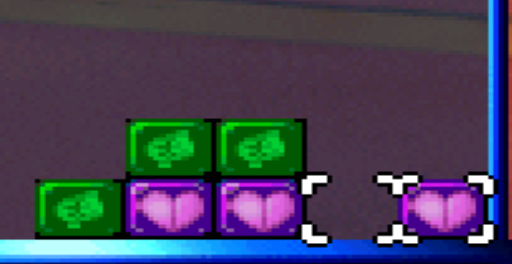
\includegraphics[width=1.3in]{chain1.png}
\end{subfigure}}\br[.5]
\centerline{$\Downarrow$}\br[.5]
\centerline{\begin{subfigure}[h]{1.3in}
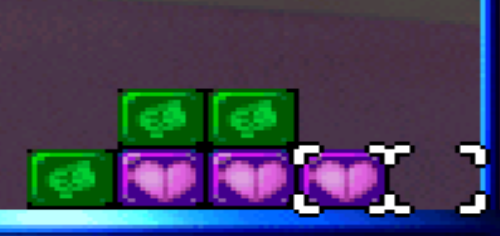
\includegraphics[width=1.3in]{chain2.png}
\end{subfigure}}\br[.5]
\centerline{$\Downarrow$}\br[.5]
\centerline{\begin{subfigure}[h]{1.3in}
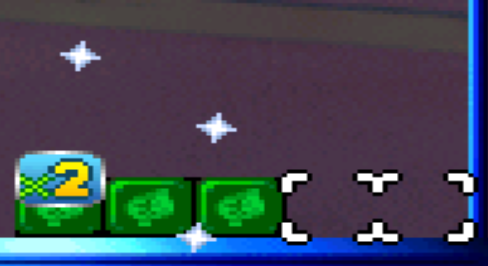
\includegraphics[width=1.3in]{chain3.png}
\end{subfigure}}
\caption{Clearing a simple $2$x chain.}
\label{fig:chain}
\end{figure}

\subsection{Task Definition}

The goal of our system is to produce an automated agent that is capable of playing Pok\'{e}mon Puzzle League at a high level. We noticed that there are many more similarities than differences between modes. In each case, the player wants to create large combos and long chains, while preventing his or her grid from reaching the top. With this in mind, we claim that optimal game strategy is largely the same in both modes, and so it is feasible to consider both cases at the same time. We will attempt to maximize our score in ``Endless'' mode and beat the in-game CPU consistently in ``Versus'' mode. We note that the in-game CPU can play at various difficulties, allowing us to record results at multiple levels.

\subsection{Oracle and Baseline}

We now give a few benchmark results. Using the game interface infrastructure explained in Sections $4$ and $5$, we quickly implemented a random AI agent which made $5$ random moves per second. This served as our baseline, and we fully expected all of our advanced algorithms (discussed in Section $6$) to beat it. For an oracle, we played the game ourselves, since we were the best game players we could find, human or machine.

Table~\ref{tab:baseline} records the performance for our baseline and oracle in $2$-player mode. We played against the in-game CPU at each level a total of $20$ times and recorded how many wins each method produced. There are five levels: Easy (E), Medium (M), Hard (H), Very Hard (VH), and Super Hard (SH). Since the game is rather complicated, the baseline AI does not do very well.

\begin{table}[ht]
\begin{center}
\begin{tabular}{c||c|c|c|c|c}
Difficulty & E & M & H & VH & SH \\ \hline\hline
Baseline & $5$ & $2$ & $0$ & $0$ & $0$ \\ \hline
Oracle & $20$ & $20$ & $19$ & $13$ & $3$
\end{tabular}
\end{center}
\caption{Baseline and oracle performance for $2$-player mode.}
\label{tab:baseline}
\end{table}

To complete our benchmark results, we also played the $1$-player mode $5$ times with each method, recording the average score achieved. Our baseline yielded an average score of $2460$, while our oracle was able to score much higher at $18781$.

\section{Approach}

Before delving into technical details, we give a high-level overview of our end-to-end system.

\subsection{System Overview}

When playing the game, we did not have access to the internal workings, memory, or data, so we could only rely on what was being displayed on screen. So, our first step involved building out an interface to the game. This allowed us to capture in-game screenshots and send movement inputs to the game at a satisfactory rate. With the interface in hand, we broke our problem down into a straightforward sequence of steps, which were to be looped until the game ended:
\begin{enumerate}
\item Capture an in-game screenshot.
\item Check if the game has ended. If so, stop.
\item Extract the agent's grid from the screenshot.
\item Calculate the best short sequence of moves possible on the grid.
\item Send the sequence of moves to the game.
\end{enumerate}
For performance reasons, it was infeasible to capture and parse a screenshot before each individual move. To compromise, we decided that calculating and executing a short sequence of $5$ to $10$ moves would still yield comparable results.

\subsection{Game State Model}

When parsing a game screenshot, it is straightforward for us to represent the board state internally as a grid that is $6$ blocks wide and $12$ blocks tall. There are a finite number of block types -- including garbage blocks and empty space -- so we can enumerate all possible values that a grid cell can take. Our model can deterministically calculate future board states after a series of moves by considering switches, clears, and falling blocks.

\section{Board Extraction}

Next, from a screenshot, we extract and classify the grid squares from the agent's board (see Appendix, Figure~\ref{fig:extract}). To do so, we used OpenCV to isolate and divide the board. We then used a logistic regression classifier to determine the type of each block. In our first implementation, our features for each block image were simply the RGB values of each pixel. However, one remaining challenge will be differentiating an active grid block from an empty background. Inspired by \cite{1}, we are hoping that to use more effective features -- for example, considering the standard deviation in color -- to solve this problem. Another challenge is that the grid varies in position, since blocks slowly rise from the bottom. To solve this, we consider the block-sized image at each possible vertical position of the lower left block. Using our classifier, we calculate the likelihood that each image is an actual block, and we pick the position that yields the highest probability.

Given a screenshot, we extract and classify the grid squares from the agent's board. To do so, we used OpenCV to isolate and divide the board. We then used a logistic regression classifier to determine the type of each block. It turns out that the best feature vector for each block image was simply taking the RGB values of each pixel, since all grid blocks of the same type always look identical. Rising blocks introduces the problem that the bottom grid is not always flush with the bottom of the game screen. To solve this, we consider the block-sized image at each possible vertical position of the lower left block. Using our classifier, we calculate the likelihood that each image is an actual block, and we pick the position that yields the highest probability. The final challenge rested in being able to differentiate the background from an actual block. As a workaround, we always chose the same game settings so that the background does not vary. Then, we divided the background itself into a grid and trained on it as well. Thus, our classifier was now able to guess the \texttt{BACKGROUND} class, which we would subsequently treat as an empty grid cell.

\section{Algorithms}
Given the game mechanics, there are several considerations that must be accounted for when deciding on an optimal algorithm:
(1) Since the game is played in real time, our algorithm for calculating an optimal set of moves must be able to return a strong set of moves relatively quickly. Consequently, an algorithm that is able to produce decent moves in a short amount of time is preferable to an algorithm that returns very strong moves but requires a large amount of processing time.
(2) The board state only changes when a swap is made. Moving the cursor around the board does not affect the position of pieces in any way. Our algorithms can thus focus on the optimal swaps, while leaving the necessary cursor movements to get there as a secondary concern.
(3) High level gameplay revolves around setting up combos and chains that can be set off by one swap. As such, it is better to attempt to find an optimal sequence of ``setup'' swaps that leads to one very influential swap, instead of trying to find optimal singleton swaps one at a time.

\textbf{TODO: Should this be moved? Now that we discuss both deterministic and random algs.} Given these considerations, we decided to explore the space of randomized algorithms that evaluate sequences of moves using a defined evaluation function. The strength of the algorithms in this space lies in their ability to quickly determine sequences of moves that yield relatively strong results. This fits our needs well since it is not necessary that we perform an exhaustive search to find a board's true optimal sequence of moves.

\subsection{Board Evaluation}

The primary goal for our board evaluation function is to give high scores to boards that contain large combos and chains and give lower scores to boards that do not result in very many pieces being cleared. In addition, since chains yield better results than combos and longer chains are the best, our evaluation function should favor long chains over large combos. We thus decided to go with a simple evaluation function that mapped this relationship directly. If we define $B$ to be a board, $S(B)$ to be the score of $B$, and $k_i$ to be the number of pieces matched and cleared at chain multiplier $i$ for the board $B$, our evaluation function is of the form:
\begin{align*}
S(B) = \sum_{i}i \cdot k_i
\end{align*}

\textbf{TODO(logan): Explain heuristics, like pressing R to raise the board, and knocking down tall columns.}

\subsection{Exhaustive Search}
A basic approach to determining an optimal move sequence is to exhaustively examine all possible combinations of moves and evaluate the resulting board states. The move sequence that yields the resulting board with the highest score according to the above defined evaluation function can then be returned as the chosen combination of moves.

The advantages of such a strategy are clear. Because all possibilites are exhaustively evaluated, this approach is guaranteed to return the true optimal sequence of moves according to the defined evaluation function. However, the primary drawback of this strategy is in its runtime. Setting up longer combos and chains generally requires several moves of preperation. Consequently, a shorter sequence of moves generally cannot result in a score that is as high as scores generated by longer move sequences. Since the exhaustive approach examines all possible board states, its runtime grows exponentially with

\subsection{Random Algorithm}

Our first approach is a Random Algorithm that works by generating a series of sequences of random board position swaps. Each sequence is then applied to the board and the board evaluation scores after each swap are summed to obtain the final score of the move sequence. The sequence which yields the highest score is returned as the chosen move sequence. The variables for this algorithm are the number of randomly generated sequences to test and the number of swaps used in a sequence. Increasing the number of tested sequences tends to yield better results at the cost of runtime. Increasing the number of moves in a sequence tends to yield larger combos and chains but also increases the runtime.
\begin{algorithm}\label{random}\small
\caption{\small Random Algorithm$(B, numTrials, numMoves)$}
$\alpha \gets 0$ \\
$\beta \gets $ empty list\\
\ForEach{$i \in $ range(0,numTrials)}{
$\alpha' \gets 0$ \\
$\beta' \gets$ generate random sequence of $numMoves$ swaps \\
\ForEach{$m \in \beta'$}{
$B \gets$ Apply $m$ to $B$ \\
$\alpha' \gets \alpha' + Evaluate(B)$
}
rollback $B$ \\
\If{$s > \alpha$}{
$\alpha \gets \alpha'$ \\
$\beta \gets \beta'$ \\
}
}
return $\alpha, \beta$
\end{algorithm}

\subsection{Genetic Algorithm}

Building upon the Random Algorithm, we decided to implement a Genetic Algorithm which attempts to combine the best parts of randomly generated move sequences in order to produce a more optimal sequence. Our Genetic Algorithm which begins by generating a set of random swap sequences, $S$. Each of these move sequences is then scored by summing the evaluation scores of the resulting board after each swap in the sequence. A new generation of sequences is then formed by selecting two sequences from $S$. During this selection process, the probability of selecting a sequence $a$ is based on the relative score of $a$ in comparison to all other sequences in $S$, with higher scores yielding higher probabilities. Once two sequences have been selected, a pivot index is picked uniformly at random. A child is generated by concatenating all the swaps up to the pivot index of one sequence with all the swaps after the pivot point of the other sequence. Thus this process generates two children. These children are added to a new sequence set $S'$ and the child generating process is continued until the size of $S'$ is equal to the size of $S$. We then set $S$ to be equal to $S'$ and repeat the process. After a specified number of generations, we return the move sequence in $S$ that yields the highest score.

Variables for this algorithm include the size of the set $S$, the number of generations to run, and the length of a move sequence. As with the Random Algorithm, increasing these parameters yields better results at the cost of increased runtime. An additional variable is the probability distribution of sequence selection based on the scores. Initial testing seems to indicate that having the selection probability be based on a distribution made up of the squares of sequence scores yields favorable results.
\begin{algorithm}\label{genetic}\small
\caption{\small Genetic Algorithm$(B, numSeq, numGen, numMoves)$}
$S \gets$ list of $numSeq$ random sequences of $numMoves$ swaps\\
\ForEach{$i \in$ range(0,numGen)}{
$S' \gets$ empty list\\
$seq1 \gets$ pick from $S$ with probability based on Evaluate() score \\
$seq2 \gets$ pick from $S$ with probability based on Evaluate() score \\
$p \gets$ uniformly random value in $range(0,numMoves)$ \\
$child1 \gets seq1[0:p] + seq2[p:numMoves]$ \\
$child2 \gets seq2[0:p] + seq1[p:numMoves]$ \\
append $child1, child2$ to $S'$ \\
$S \gets S'$
}
return sequence in $S$ with best Evaluate() score\\
\end{algorithm}

\section{Results and Analysis}

\section{Conclusion}

\subsection{Future Work}

\section{Appendix}
A video demonstration of our AI agent in $2$-player mode has been uploaded to YouTube at \href{https://www.youtube.com}{https://www.youtube.com}.

% \begin{figure}[h]
% \begin{center}
% \begin{subfigure}[h]{3.2in}
% 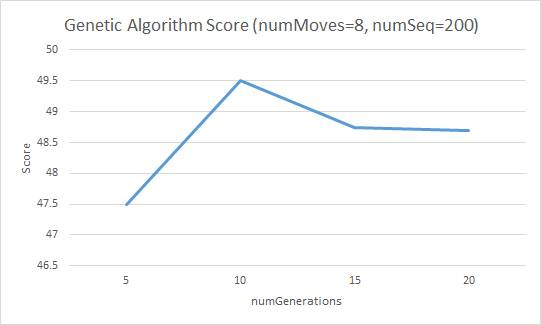
\includegraphics[width=3.2in]{geneticScore.jpg}
% \end{subfigure}
% \begin{subfigure}[h]{3.2in}
% 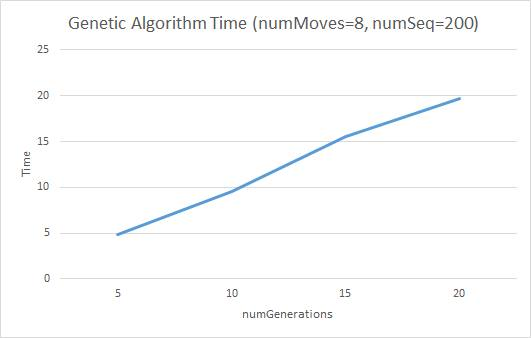
\includegraphics[width=3.2in]{geneticTime.jpg}
% \end{subfigure}
% \caption{Score and runtime as functions of the number of generations used in the Genetic Algorithm.}
% \label{fig:genetics}
% \end{center}
% \end{figure}

% \begin{figure}[ht!]
% \centerline{
% \begin{subfigure}[h]{1.3in}
% 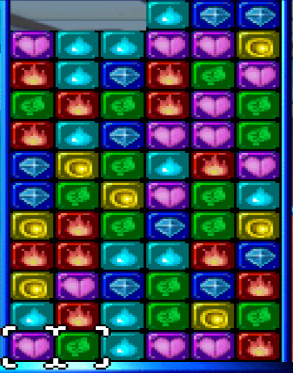
\includegraphics[width=1.3in]{inspirational1.png}
% \caption*{Start: $(0,0)$}
% \end{subfigure}
% ~$\mathbf{\Longrightarrow}$~
% \begin{subfigure}[h]{1.3in}
% 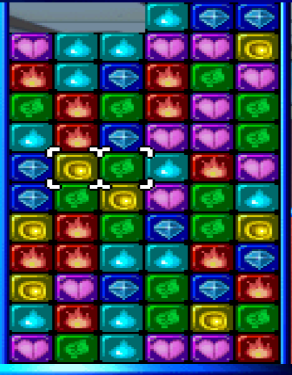
\includegraphics[width=1.3in]{inspirational2.png}
% \caption*{Red-blue: $(7,0)$}
% \end{subfigure}
% ~$\mathbf{\Longrightarrow}$~
% \begin{subfigure}[h]{1.3in}
% 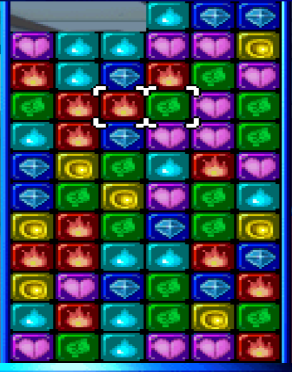
\includegraphics[width=1.3in]{inspirational3.png}
% \caption*{Green-red: $(8,2)$}
% \end{subfigure}
% ~$\mathbf{\Longrightarrow}$~
% \begin{subfigure}[h]{1.3in}
% 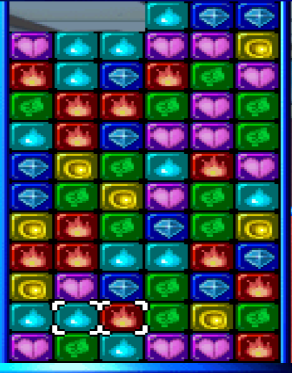
\includegraphics[width=1.3in]{inspirational4.png}
% \caption*{Red-blue: $(1,1)$}
% \end{subfigure}}\end{figure}

\begin{thebibliography}{1}
\bibitem{1} P. Frey, D. Slate. Letter Recognition using Holland-Style Adaptive Classifiers. ML, 1991.
\bibitem{2} C. Thiery, B. Scherrer. Building Controllers for Tetris. ICGA, 2009.
\end{thebibliography}

\end{document}